\documentclass[12pt]{article} % use larger type; default would be 10pt

%packages
\usepackage[utf8]{inputenc} % set input encoding (not needed with XeLaTeX)
\usepackage{fancyhdr}
\usepackage{float}
\usepackage{geometry}
\usepackage{ulem}
\usepackage{soul}
\usepackage{color}
\usepackage{graphicx}
\usepackage{hyperref}
\usepackage{array}
\usepackage{caption}
\usepackage{titling}
\usepackage{enumerate} 
\usepackage[dvipsnames]{xcolor}
\usepackage{amsmath}
\usepackage{amssymb}
\usepackage[compact]{titlesec}


 %put box around figure captions
\makeatletter
\long\def\@makecaption#1#2{%
  \vskip\abovecaptionskip
  \sbox\@tempboxa{\fbox{#1: #2}}%
  \ifdim \wd\@tempboxa >\hsize
    \fbox{\parbox{\dimexpr\linewidth-2\fboxsep-2\fboxrule}{#1: #2}}\par
  \else
    \global \@minipagefalse
    \hb@xt@\hsize{\hfil\box\@tempboxa\hfil}%
  \fi
  \vskip\belowcaptionskip}
\makeatother

%reduce space between 
\titlespacing{\section}{0pt}{*1}{*0}
\titlespacing{\subsection}{0pt}{*1}{*0}
\titlespacing{\subsubsection}{0pt}{*0}{*0}


%no indent and modify distance between paragraphs
\setlength\parindent{0pt}
\setlength\parskip{12pt}

%set margins and line spacing
\geometry{margin=1in}
\linespread{1.2}
\geometry{letterpaper}

%math operators
\DeclareMathOperator{\E}{\mathbb{E}}

%set up header and page numbering
\pagestyle{fancy}
\lhead{CS 155 Final}
\rhead{Timothy Liu}
\pagenumbering{arabic}



\title{CS155 Final}
\author{Timothy Liu}

\begin{document}


\maketitle

\section{Problem 1}
\subsection{Question A}
True.
\subsection{Question B}
Option B
\subsection{Question C}
K1: middle image\\
K2: rightmost image\\
K3: leftmost image
\subsection{Question D}
Option B y = 2.
\subsection{Question E}
Option B
\subsection{Question F}
True
\subsection{Question G}
Option A
\subsection{Question H}
False
\subsection{Question I}
True
\subsection{Question J}
False
\subsection{Question K}
Option B
\subsection{Question L}
True
\subsection{Question M}
True
\subsection{Question N}
True

\section{Problem 2}
\subsection{Question 1}

\begin{figure}[H]
	\makebox[\textwidth][c]{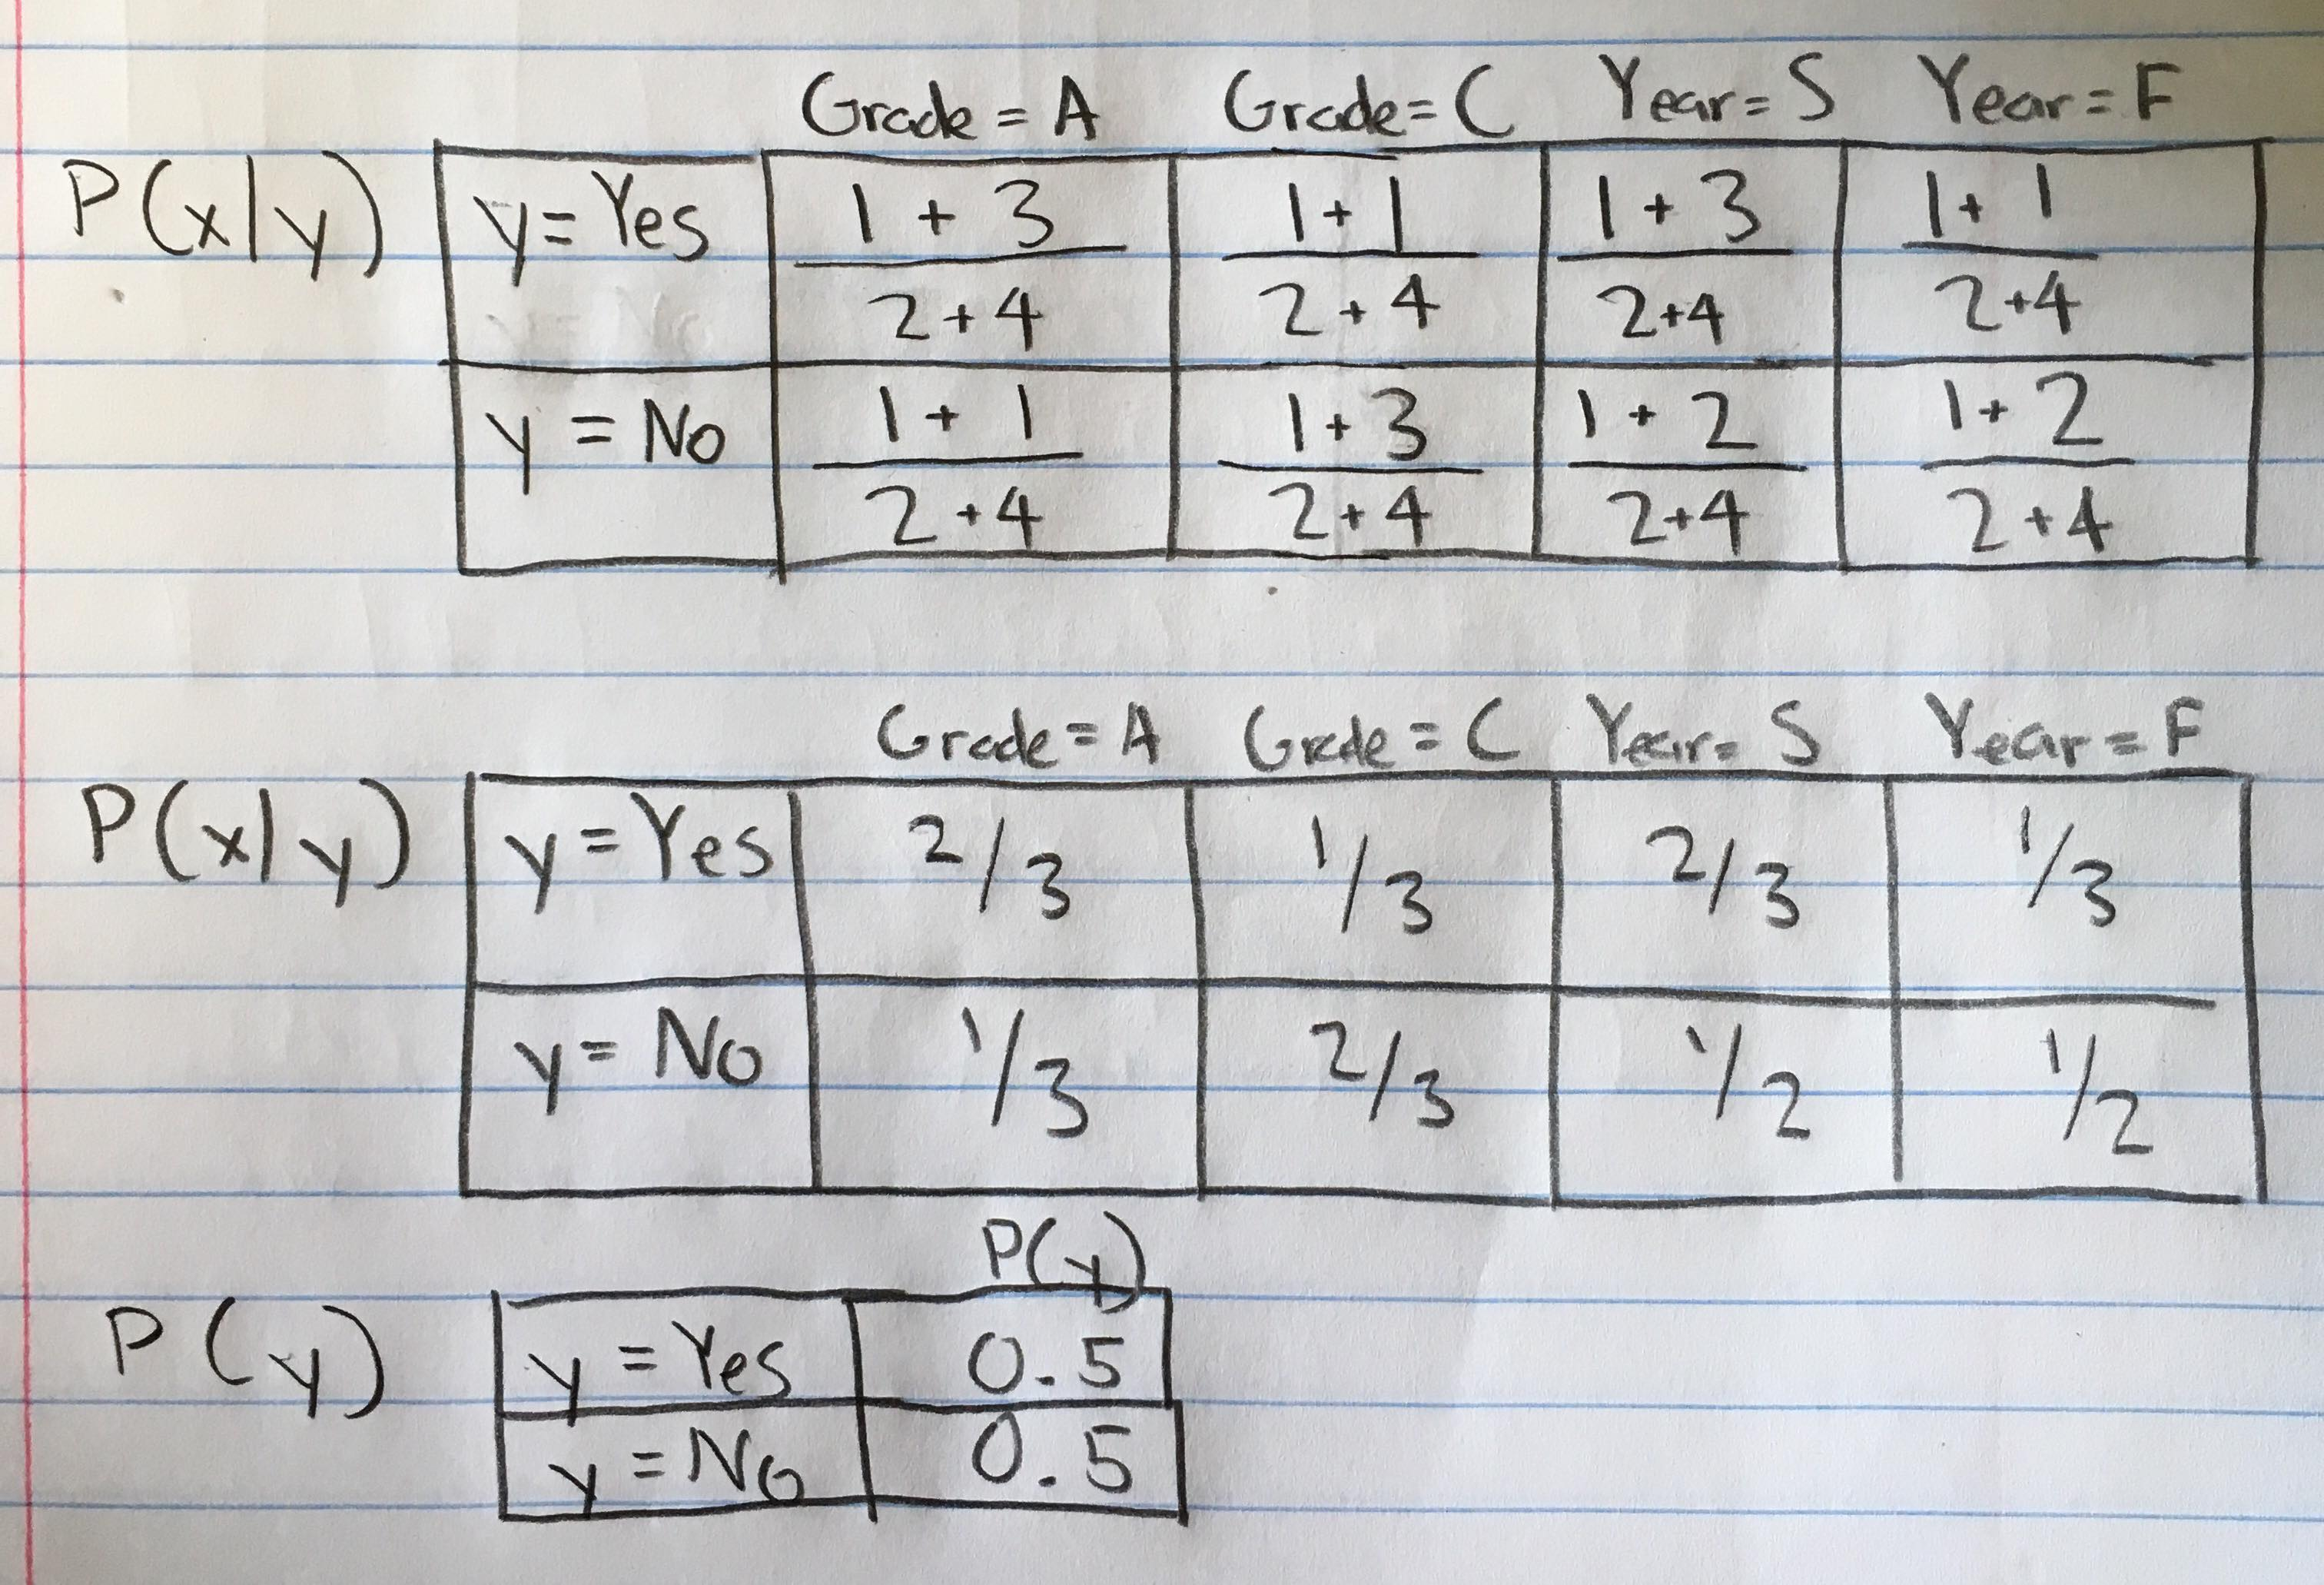
\includegraphics[width=5in]{2_1.jpg}}
	\vspace{-10mm}
	\caption{Naive Bayes model parameters.}
\end{figure}

\subsection{Question 2}
P(Year = Freshman, Grade = C, Happy = No) =\\ $P(Happy = No) \times P(Grade = C|Happy = No) \times P(Year = Freshman| Happy = No)=\\
\frac{1}{2} \times \frac{2}{3} \times \frac{1}{2} = \frac{1}{6}$

\subsection{Question 3}
\begin{figure}[H]
	\makebox[\textwidth][c]{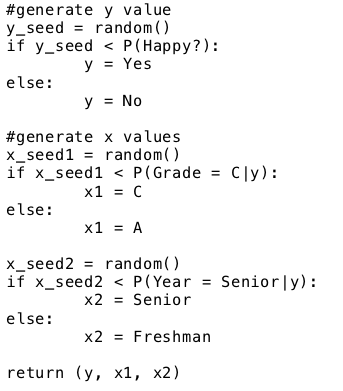
\includegraphics[width=4in]{2_3.png}}
	\vspace{-10mm}
	\caption{Pseudocode for drawing from a trained model given the parameters have been calculated..}
\end{figure}

\section{Problem 3}
\subsection{Question 3}
\begin{figure}[H]
	\makebox[\textwidth][c]{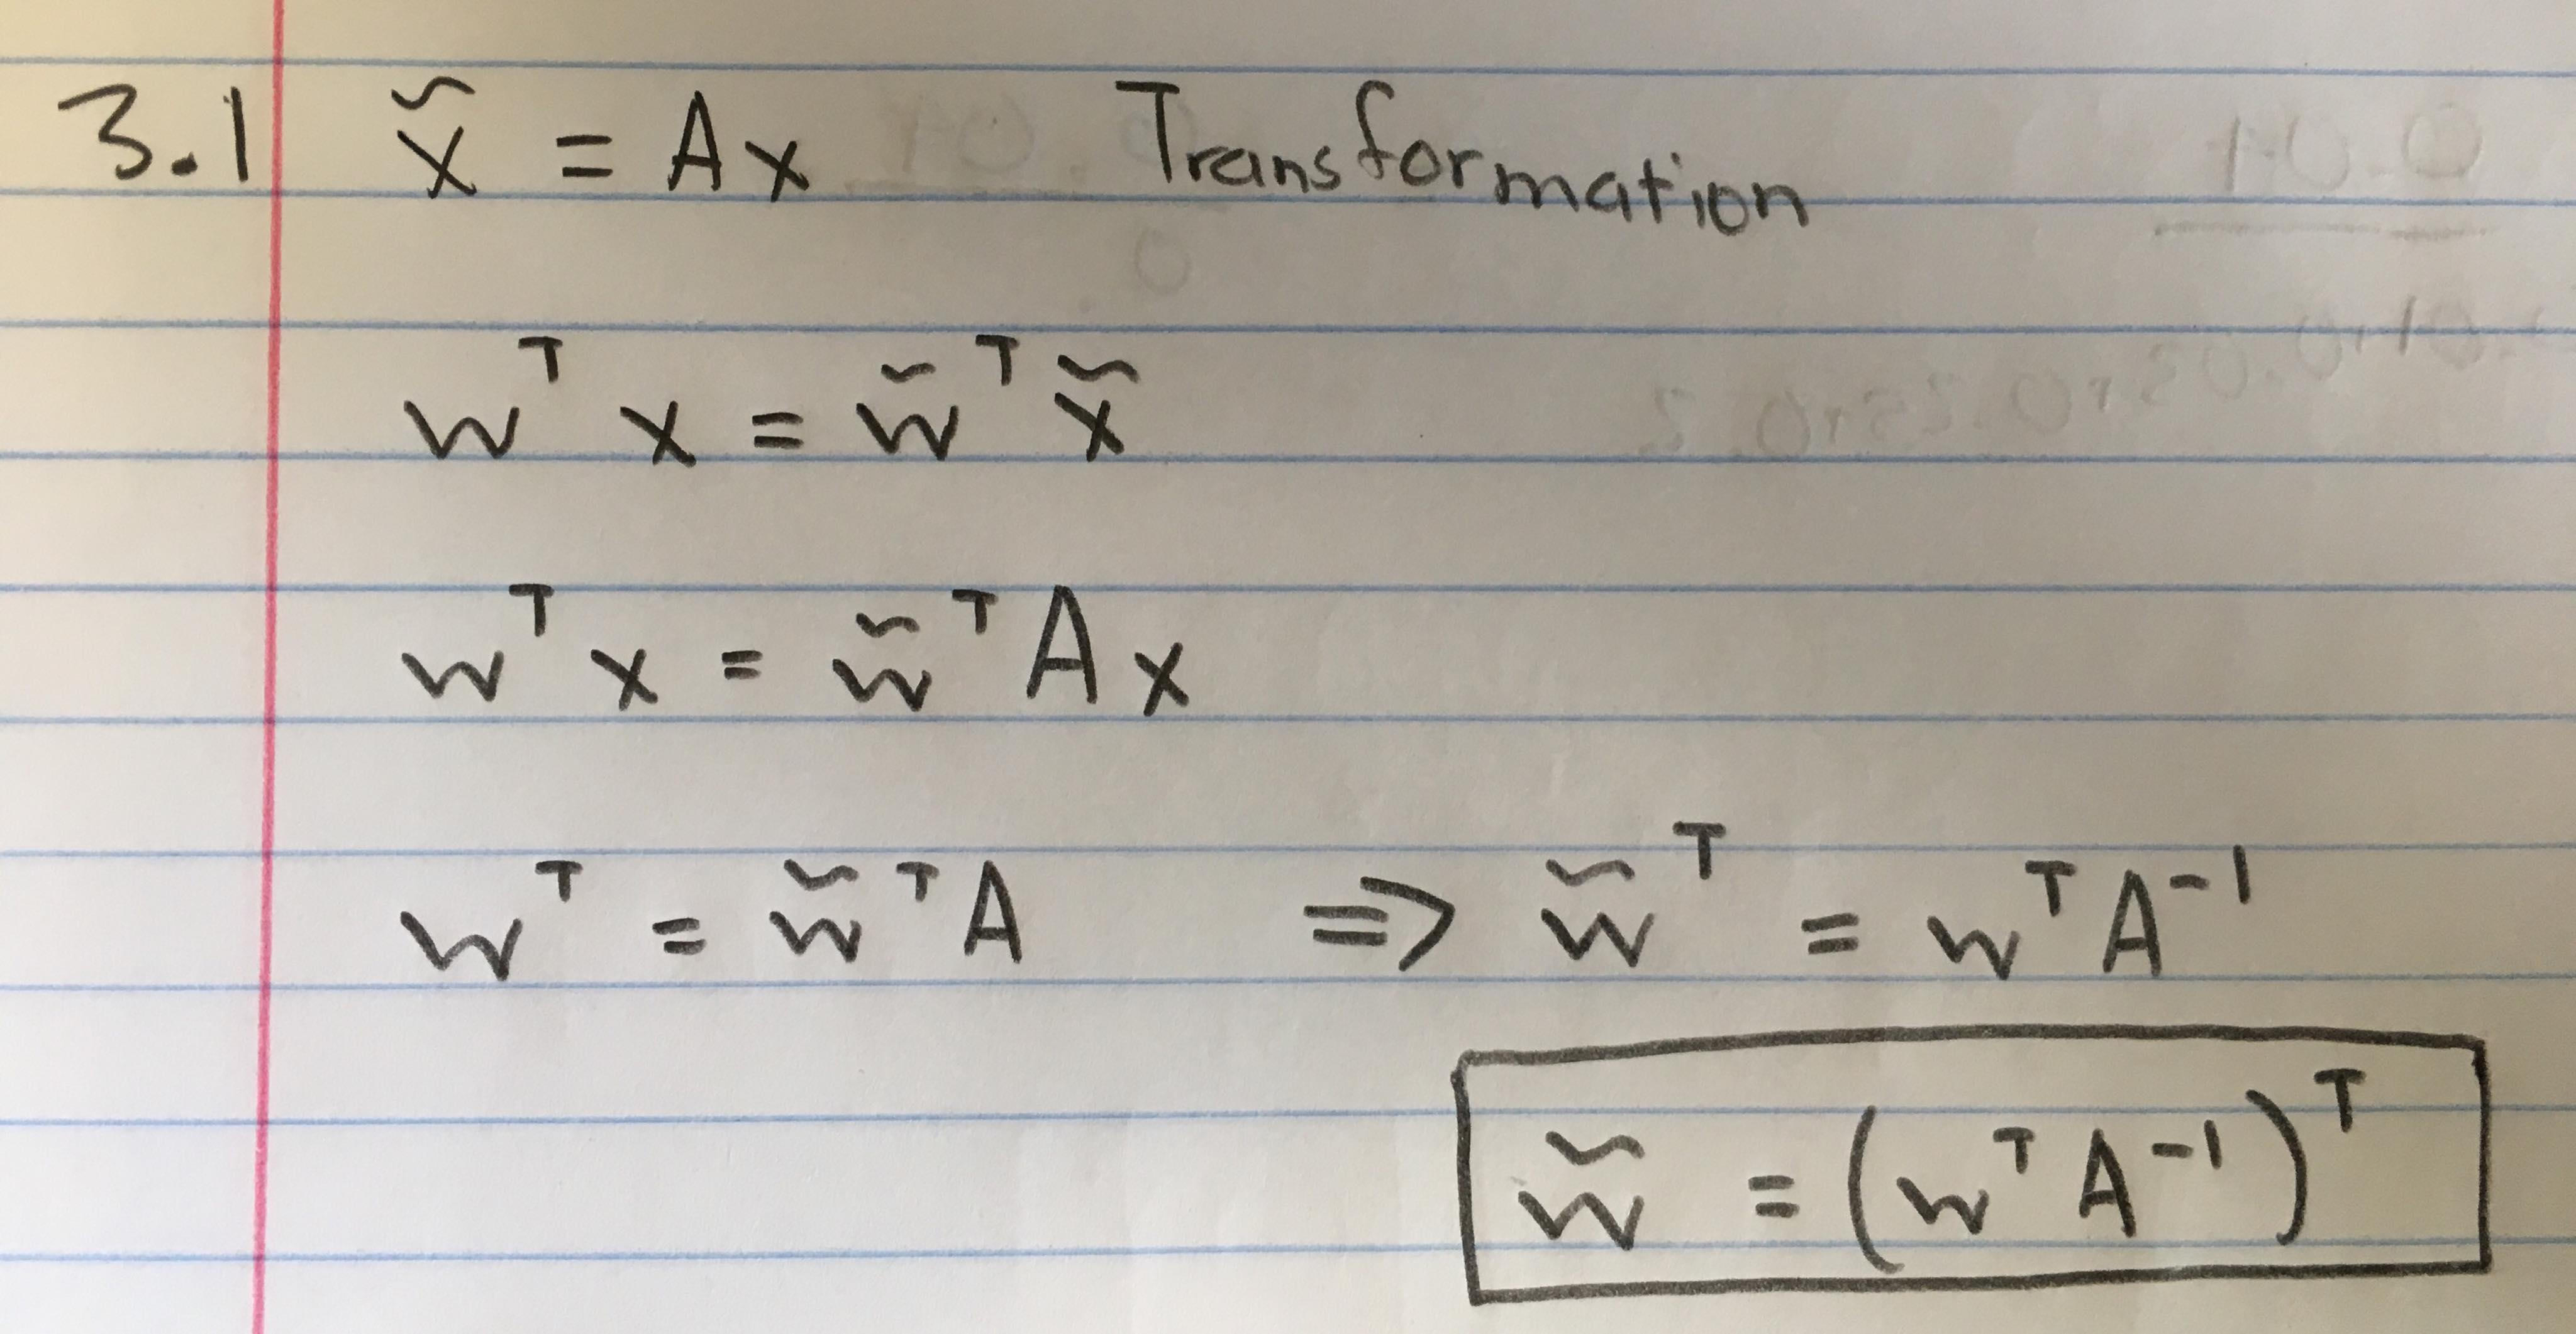
\includegraphics[width=4in]{3_1.jpg}}
	\vspace{-10mm}
\end{figure}

\subsection{Question 2}
\begin{figure}[H]
	\makebox[\textwidth][c]{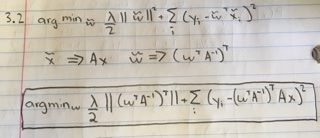
\includegraphics[width=5in]{3_2.jpg}}
	\vspace{-10mm}
\end{figure}

\subsection{Question 3}
When A is a rescaling matrix, its effect on the weight matrix in Question 1 is to also rescale it. Standard ridge regression is impacted only by the parameter $\lambda$ which only appears outside of the summation. The $\lambda$ puts  a constrain on the norm of the weight vector. The answer from Question 2 changes the weight vector inside and outside of the summation. Adding A to the inside means the error that we are trying to minimize is also affected by how far the predicted value is from the true value through A. Ridge regression does not have any impact on the accuracy of the weight vector, only the norm. The answer to Question 2 affects both.

\section{Problem 4}

\subsection{Question 1}
U and V are selected to maximize P(S). At worse, U and V can both be equal to X, which would make P(S) for the dual point model equivalent to P(S) for the single point model. However, U and V can be selected more optimally, and having two vectors allows greater freedom to choose U and V to maximize P(S). Thus, the data likelihood for the dual-point model is never less than that of the single-point model.

\subsection{Question 2}
This would imply that U, V, and X are all equivalent to each other and that the dual point and single point models are the same. 

\section{Problem 5}

\subsection{Question 1}
\begin{figure}[H]
	\makebox[\textwidth][c]{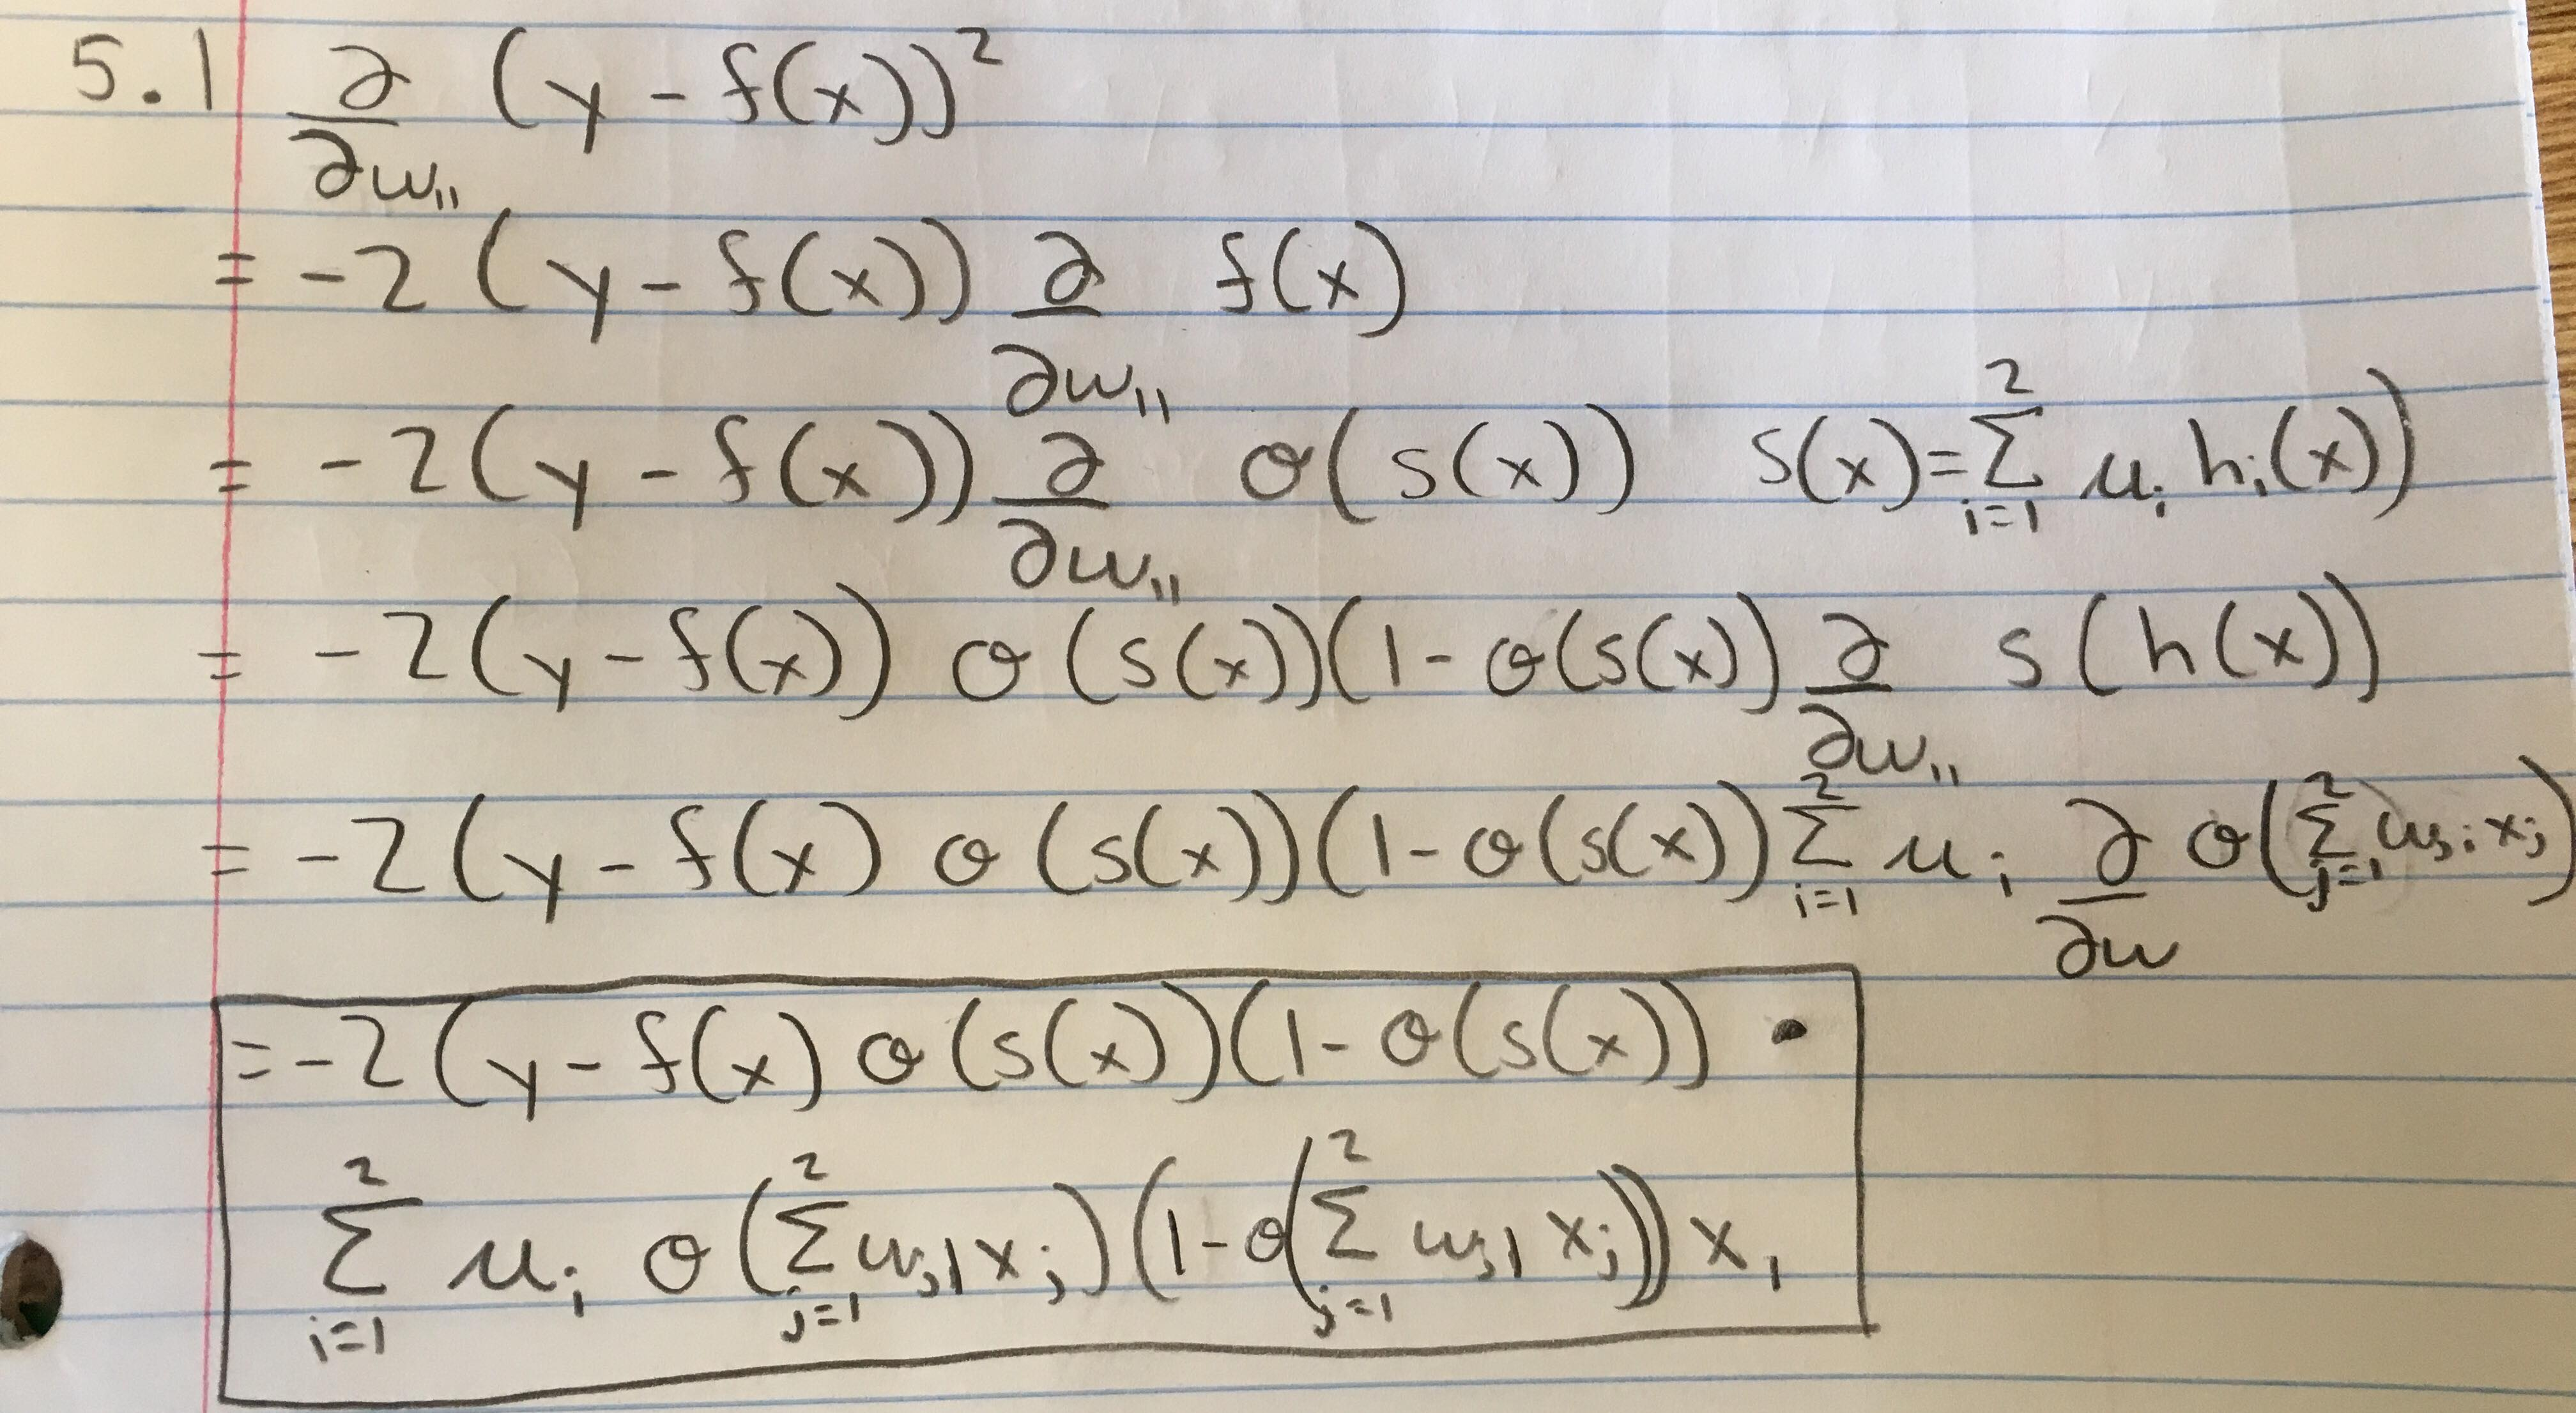
\includegraphics[width=5in]{5_1.jpg}}
	\vspace{-10mm}
\end{figure}

\subsection{Question 2}
\begin{figure}[H]
	\makebox[\textwidth][c]{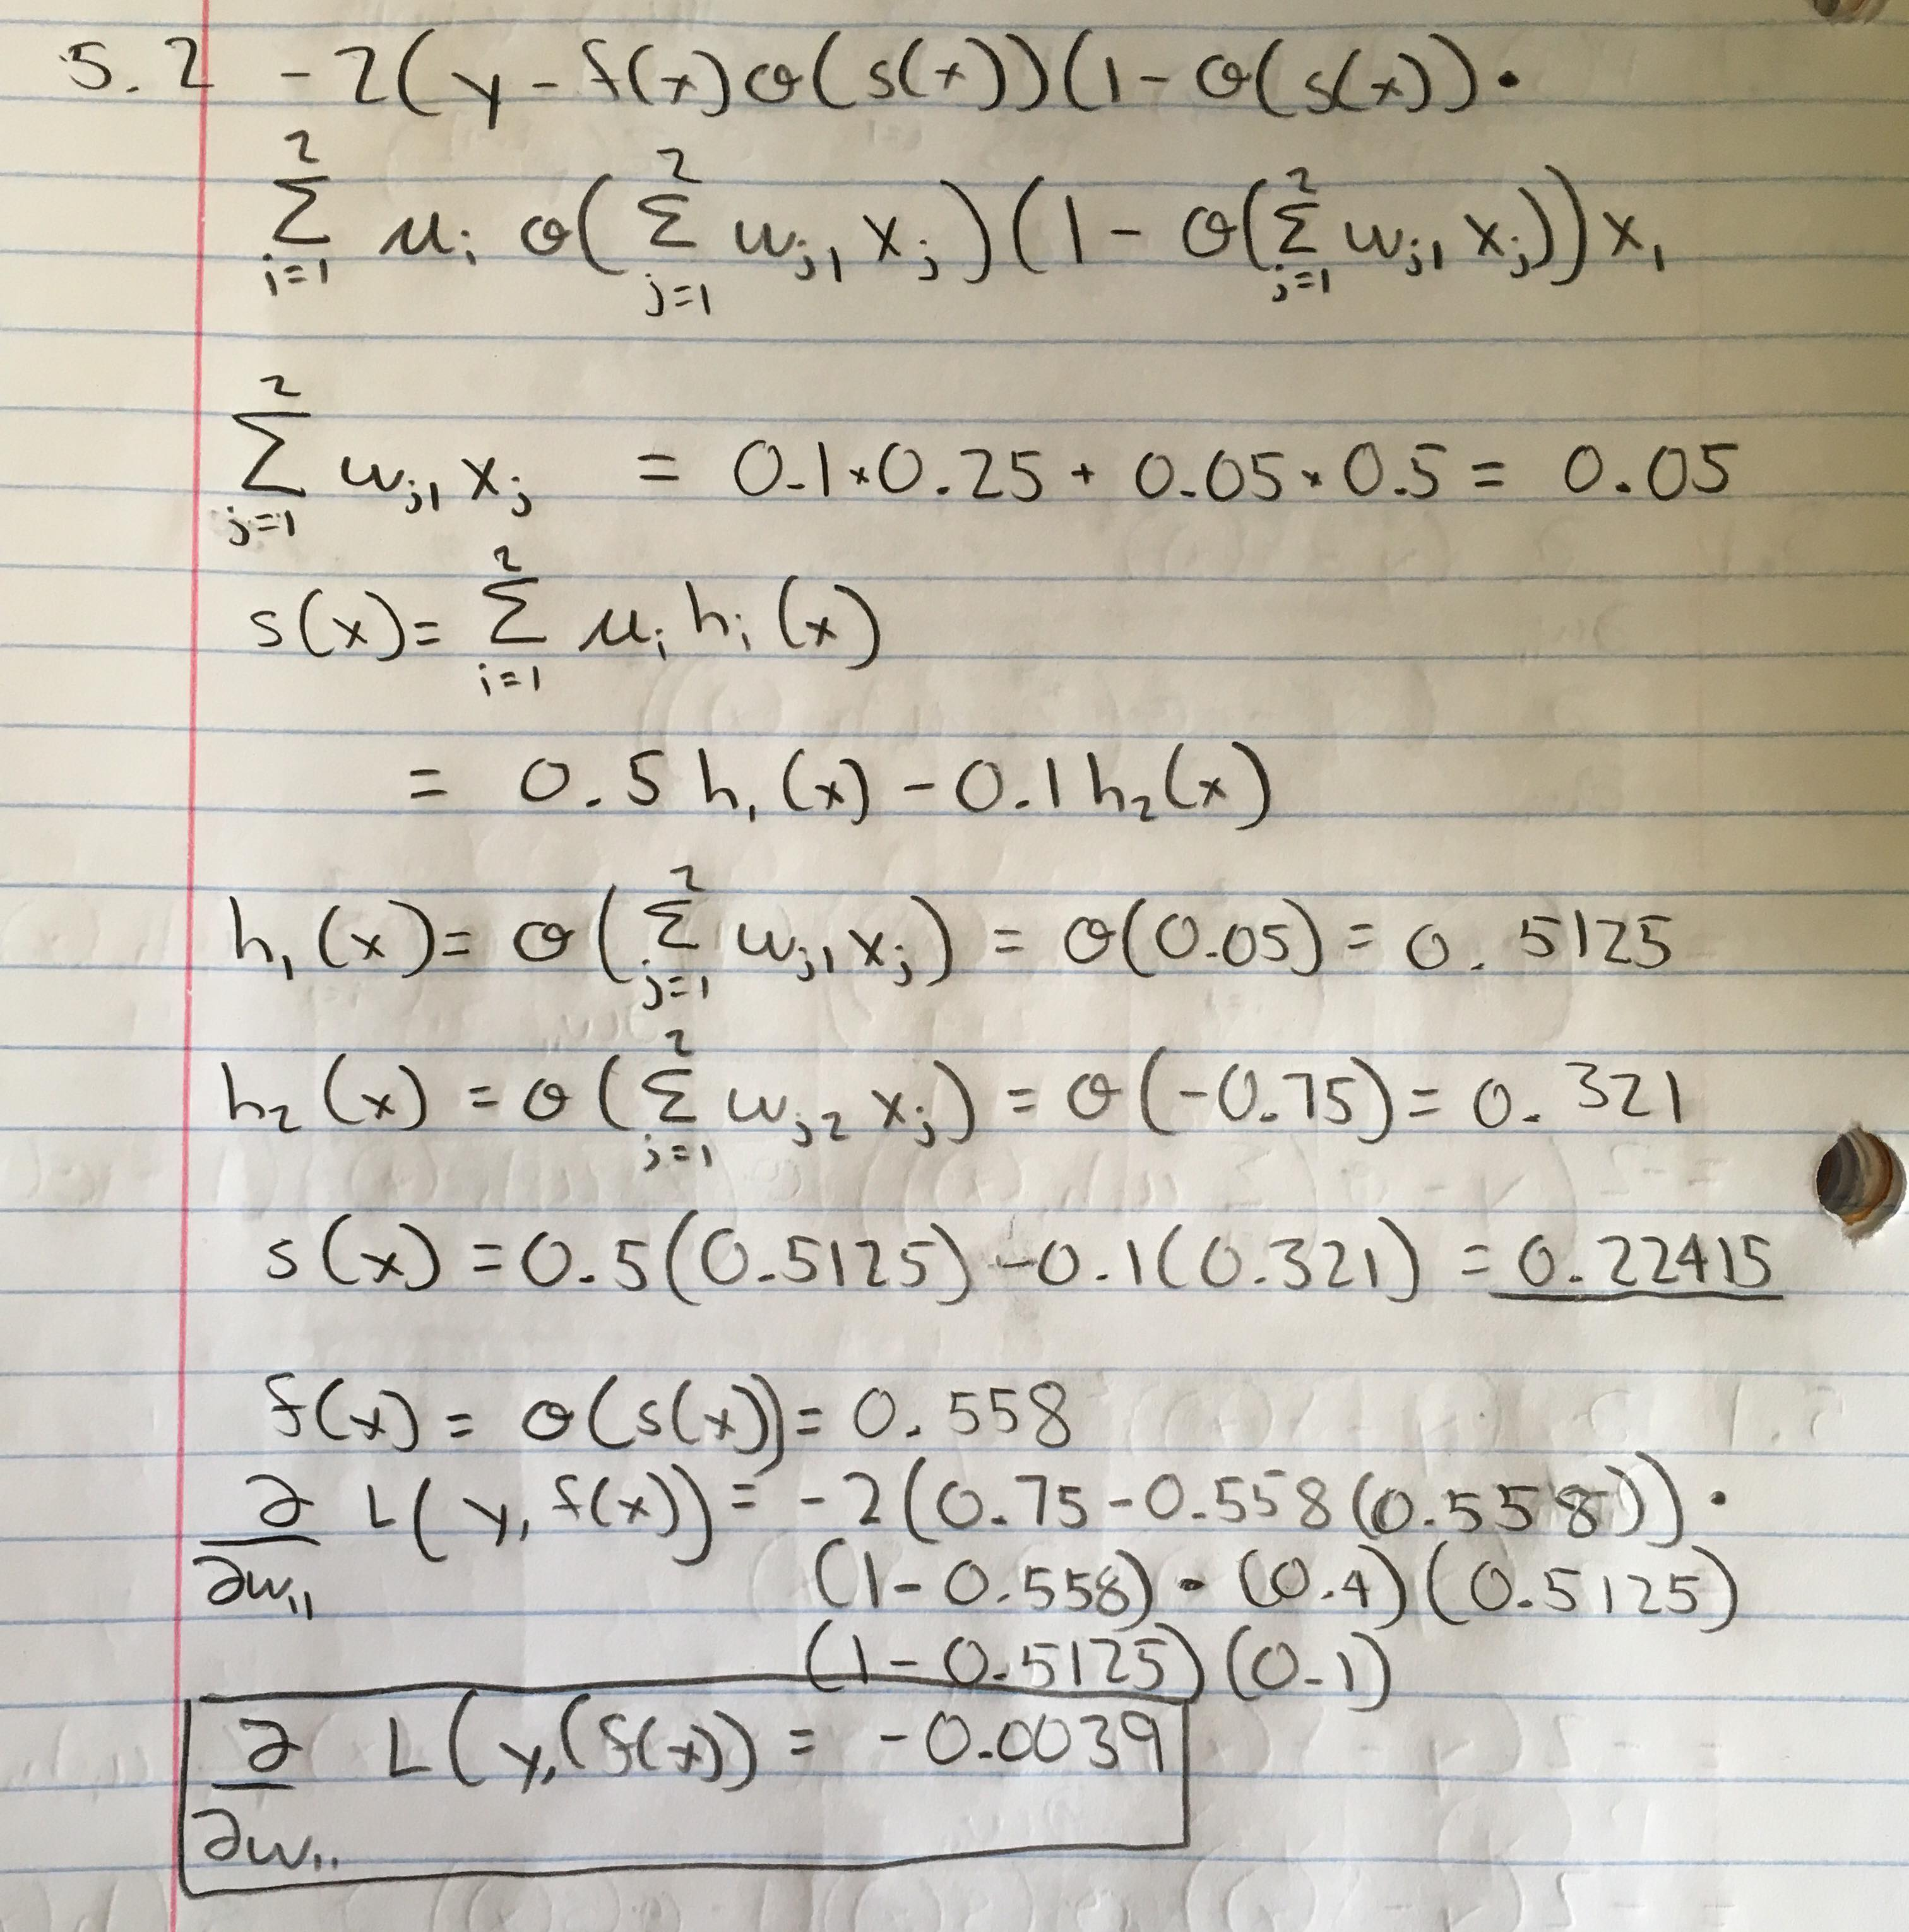
\includegraphics[width=5in]{5_2.jpg}}
	\vspace{-10mm}
\end{figure}

\subsection{Question 3}
The sigmoid term at the output of each adder results in the vanishing gradient problem. Any value far away from 0 has a small gradient. The problem worsens with multiple layers because the gradient is multiplied by several values that are close to zero, since each layer has its own sigmoid.







\end{document}
